%
% sin2.tex
%
% (c) 2024 Prof Dr Andreas Müller
%
\begin{figure}
\centering
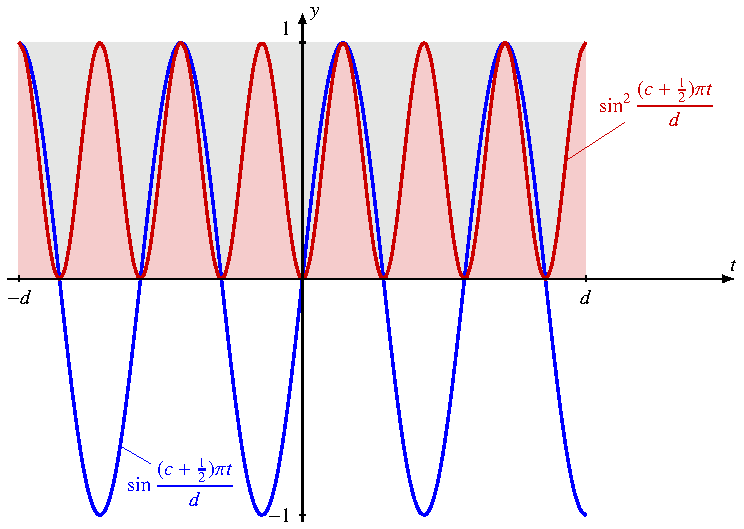
\includegraphics{chapters/060-variation2/images/sin2.pdf}
\caption{Graphischer Beweis des Lemmas~\ref{buch:variation2:legendre:lemma:sin}.
Der Graph der Funktion $t\mapsto\sin^2((c+\frac12)\pi t)/d)$
halbiert das Rechteck mit den Ecken $(-d,0)$ und $(d,1)$,
die rote Fläche unter dem Graphen ist daher $d$.
\label{buch:variation2:legendre:fig:sin2}}
\end{figure}

